\documentclass[aspectratio=169,10pt]{beamer}
\usetheme{Madrid}
\usepackage{graphicx}
\usepackage{amssymb}

% Tắt shadow
\setbeamertemplate{blocks}[rounded][shadow=false]
\setbeamertemplate{navigation symbols}{}

% Color configuration
\definecolor{primaryblue}{RGB}{20, 55, 110}
\setbeamercolor{palette primary}{bg=primaryblue,fg=white}
\setbeamercolor{structure}{fg=primaryblue}

\begin{document}

\begin{frame}{Question: How Can We Plot a 3D Surface?}
    \begin{columns}[T]
        % Cột trái: 3 bước phác họa đồ thị 3D
        \begin{column}{0.54\textwidth}
            \begin{block}{Step-by-Step Sketching Method}
                \small
                To draw a surface $z = f(x, y)$, we reconstruct it from 2D slices:
                \begin{enumerate}
                    \item \textbf{Step 1 (2D Level Curves)}: On the $xy$-plane, draw curves for multiple constant heights $f(x, y) = k$.
                    \item \textbf{Step 2 (Lift to 3D)}: In $Oxyz$ space, lift each 2D curve up to its actual height $z = k$.
                    \item \textbf{Step 3 (Form 3D Surface)}: Connect/loft the curves together with a smooth surface mesh.
                \end{enumerate}
            \end{block}
        \end{column}

        % Cột phải: Animation trực quan hóa 3 bước vẽ
        \begin{column}{0.44\textwidth}
            \centering
            \vspace{0.1cm}
            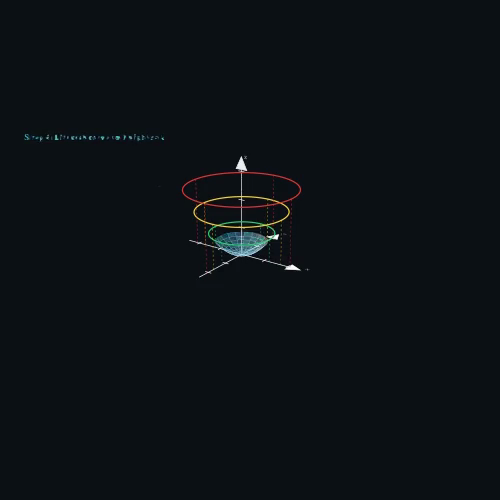
\includegraphics[width=0.92\linewidth, keepaspectratio]{HowToPlotSurfaceScene.png}
            
            \vspace{0.1cm}
            {\tiny \textcolor{gray}{\textit{Step 1: Draw 2D $\to$ Step 2: Lift to $z=k$ $\to$ Step 3: Form Surface}}}
        \end{column}
    \end{columns}
\end{frame}

\end{document}
